
The system allows farmers to access the personalized best practice data based on their location and type of production. To analyze farmers' performance, they are required to insert production information periodically. The system provides pages where they can exchange their opinion among farmers and ask suggestions to agronomists by sending messages. 
\newline
\newline
On the other hand, the system serves agronomists to let them answer the requests from farmers. 
Agronomists need to specify which areas are under their responsibility; then, according to the registered areas, the system organizes the visits plan and notify them. The provided plans can be modified by the agronomist if necessary, and the meetings status will be also tracked.
\newline
\newline
Lastly, for policy maker, the system provides the classification of farmer according to their performance, places with critical natural disaster. Assignment of incentives and request of writing good practices on selected farmers will be also managed. To track the effectiveness of the steering initiatives carried out by farmers and agronomists, commitments from them will be accessible.
\newline
\newline
Considering their jobs, since farmers and agronomists need to be outside most of the time, using smartphone application would be suitable for them by the aspect of portability. Instead policy makers are supposed to work mainly inside; therefore, the desktop based web application will be provided. 
\newline
\newline
Here we would like to introduce a few images to show how the application looks like on main functions. Figure \ref{fig:FE_image1} shows "sign up" and "sign in" pages, which are common for all types of user. Figure \ref{fig:FE_image2} serves for farmers to let them insert the production results. The third figure \ref{fig:FE_image3} shows the process of forum creation. Farmers can update their production data from there.
Then forth figure \ref{fig:FE_image4} works for agronomists, it shows their daily plan and let them edit according to their needs. Lastly, figures \ref{fig:FE_image5} visualise the different kind of plots to show the effectiveness of initiatives done by agronomists to sustain farmers' activities. We will present other mock-ups and more detailed ones in our Design Document. 

\newpage
\begin{figure}[H]
	\centering
    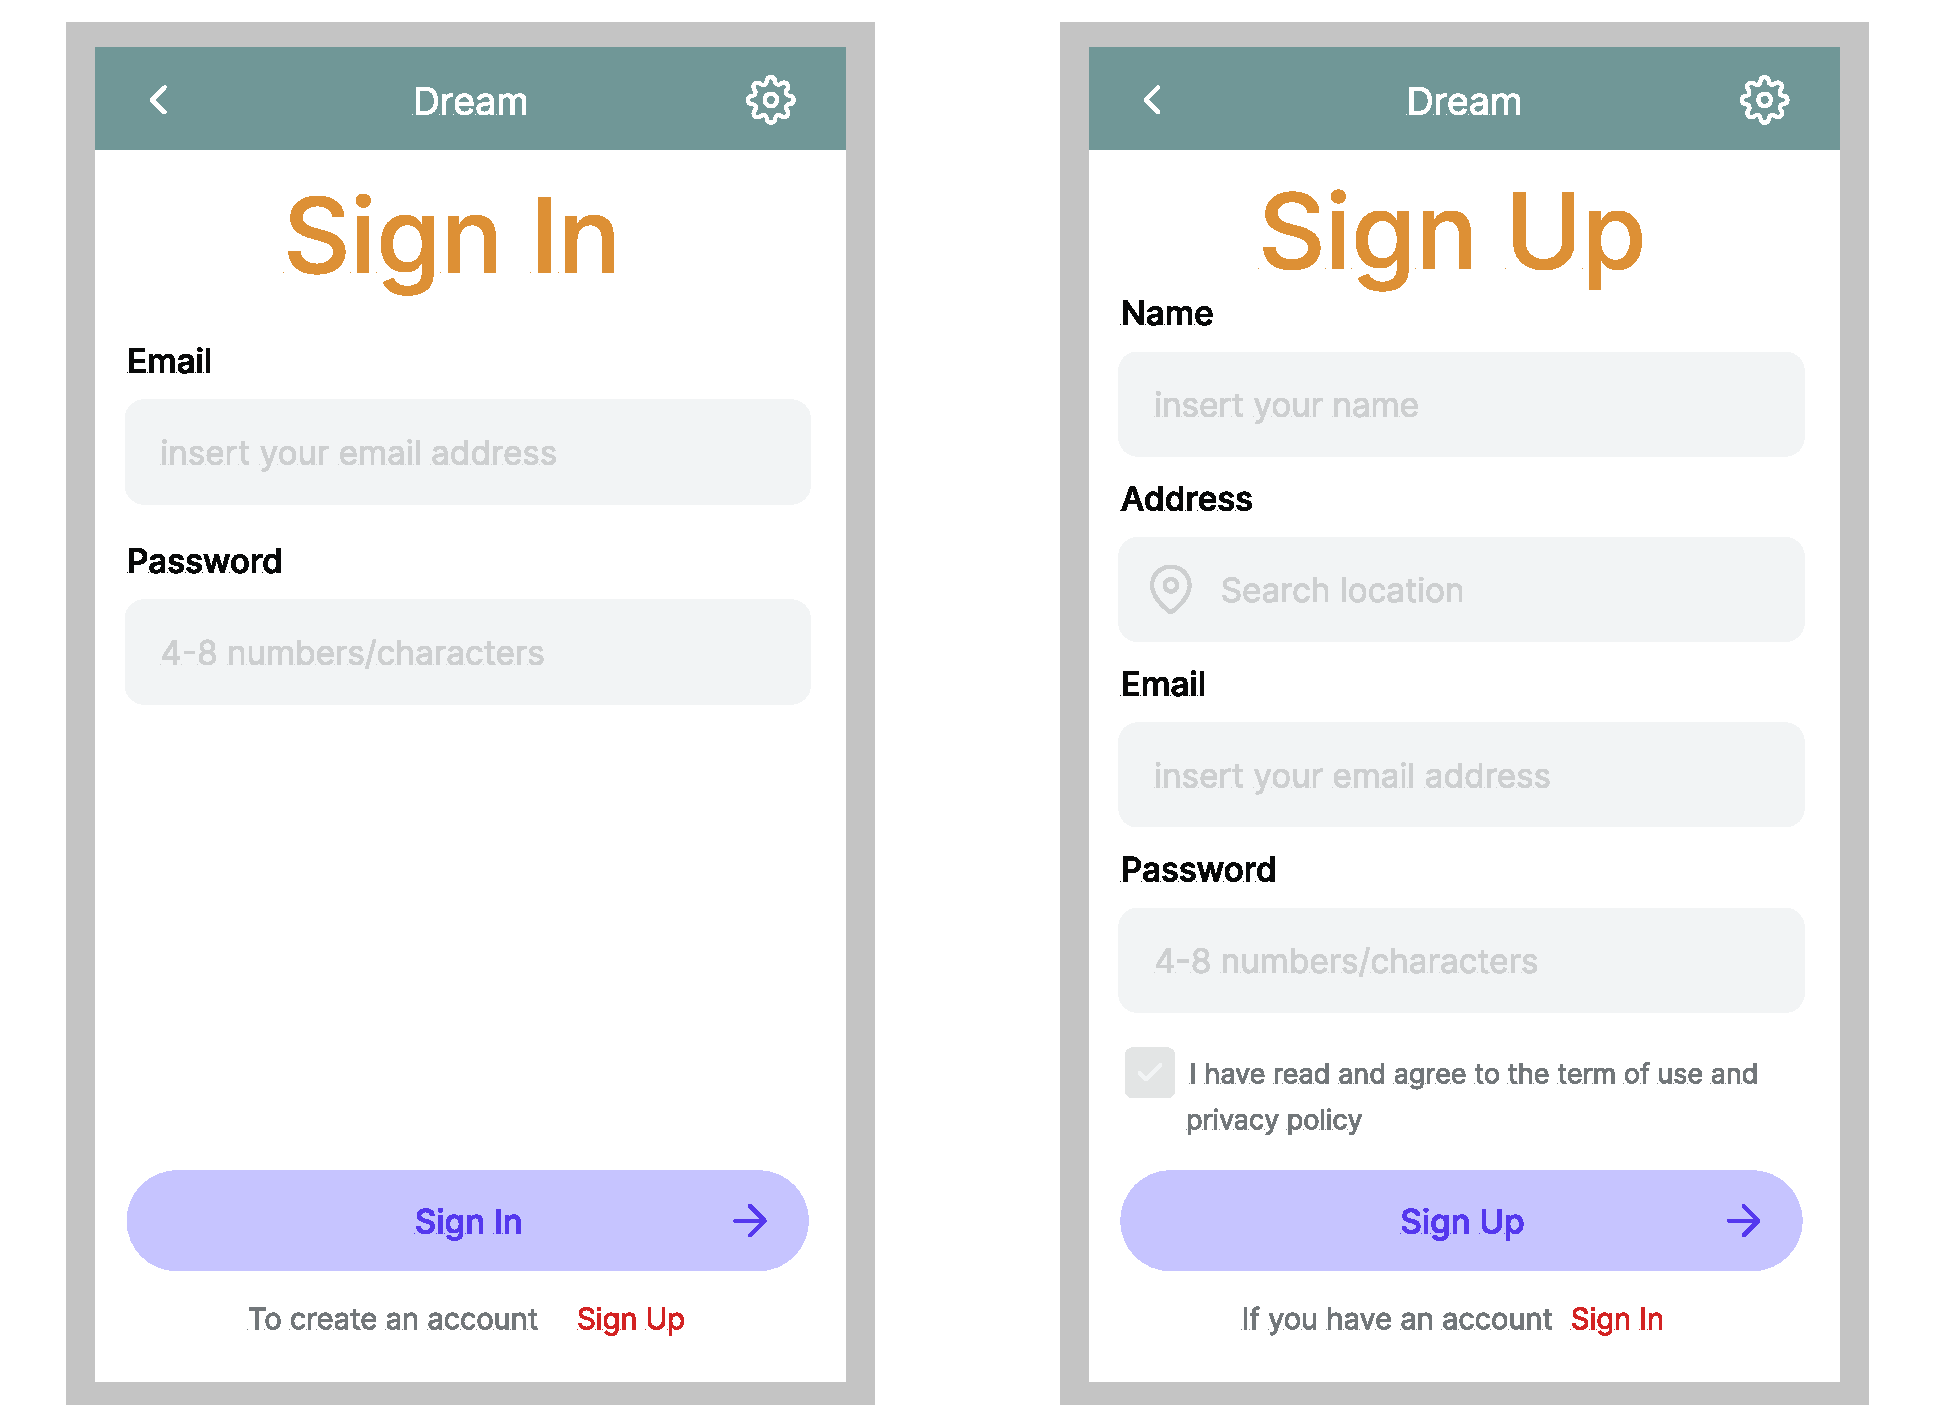
\includegraphics[page=1, width=0.8\textwidth]{Images/UI/sign_up_in.pdf}

	\caption{\label{fig:FE_image1}Sign In, Sign Up}

\end{figure}

\begin{figure}[H]
	\centering
    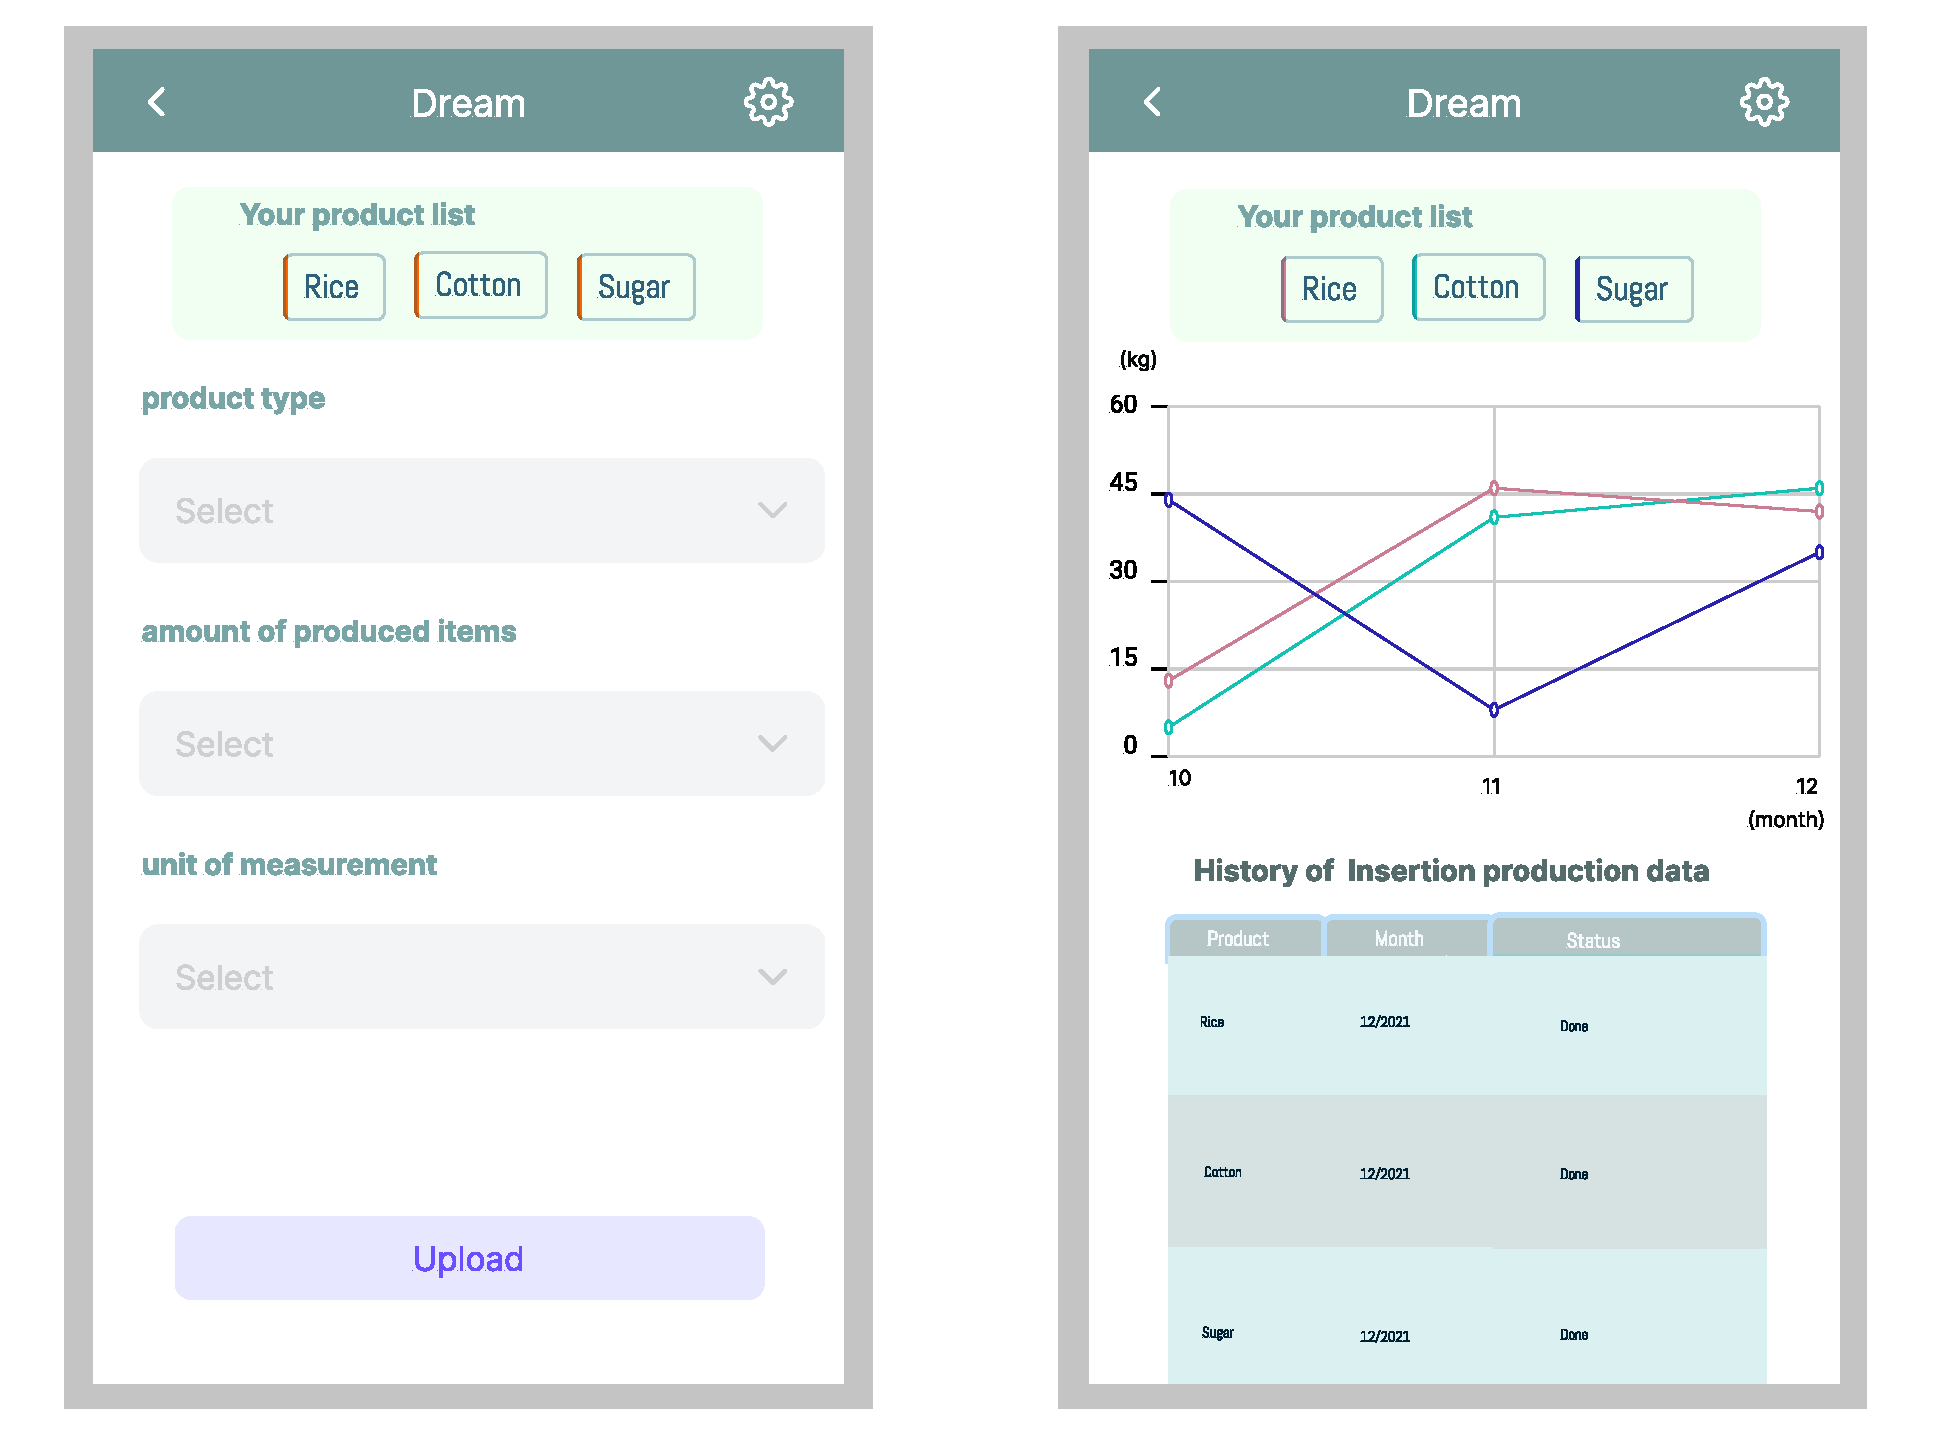
\includegraphics[width=0.8\columnwidth]{Images/UI/product_amount_registration.pdf}
	\caption{\label{fig:FE_image2}Product registration, Amount registration}

\end{figure}



\begin{figure}[H]
	\centering
    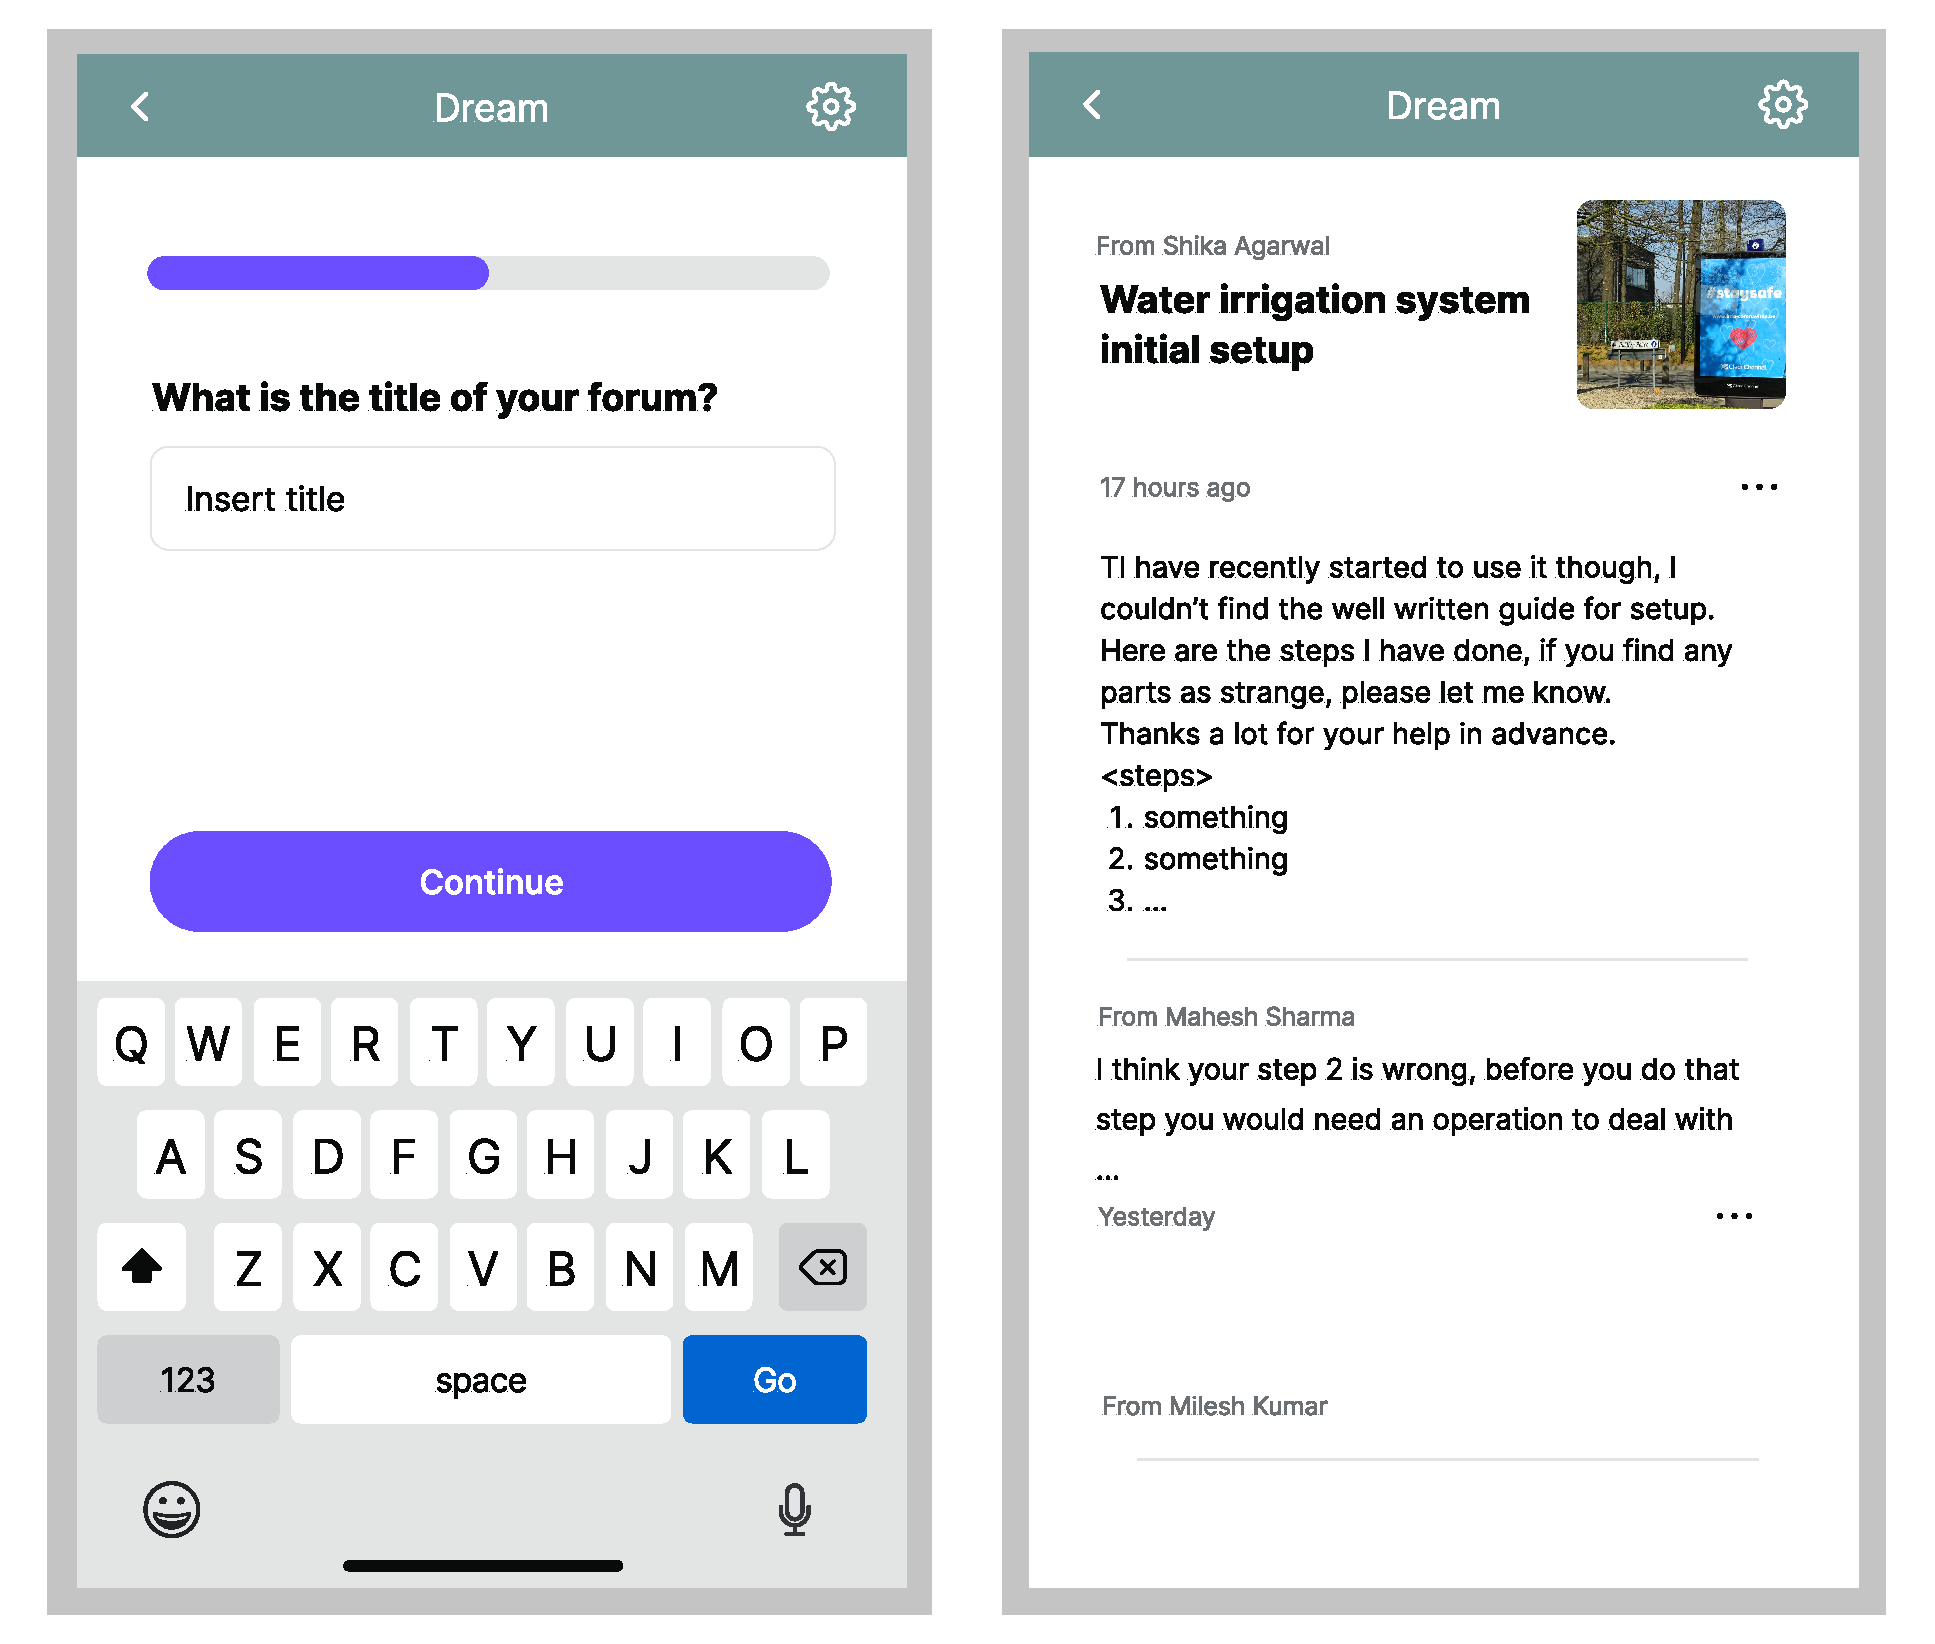
\includegraphics[width=0.8\columnwidth]{Images/UI/forum.pdf}
	\caption{\label{fig:FE_image3}Forum insertion, visualisation}

\end{figure}

\begin{figure}[H]
	\centering
    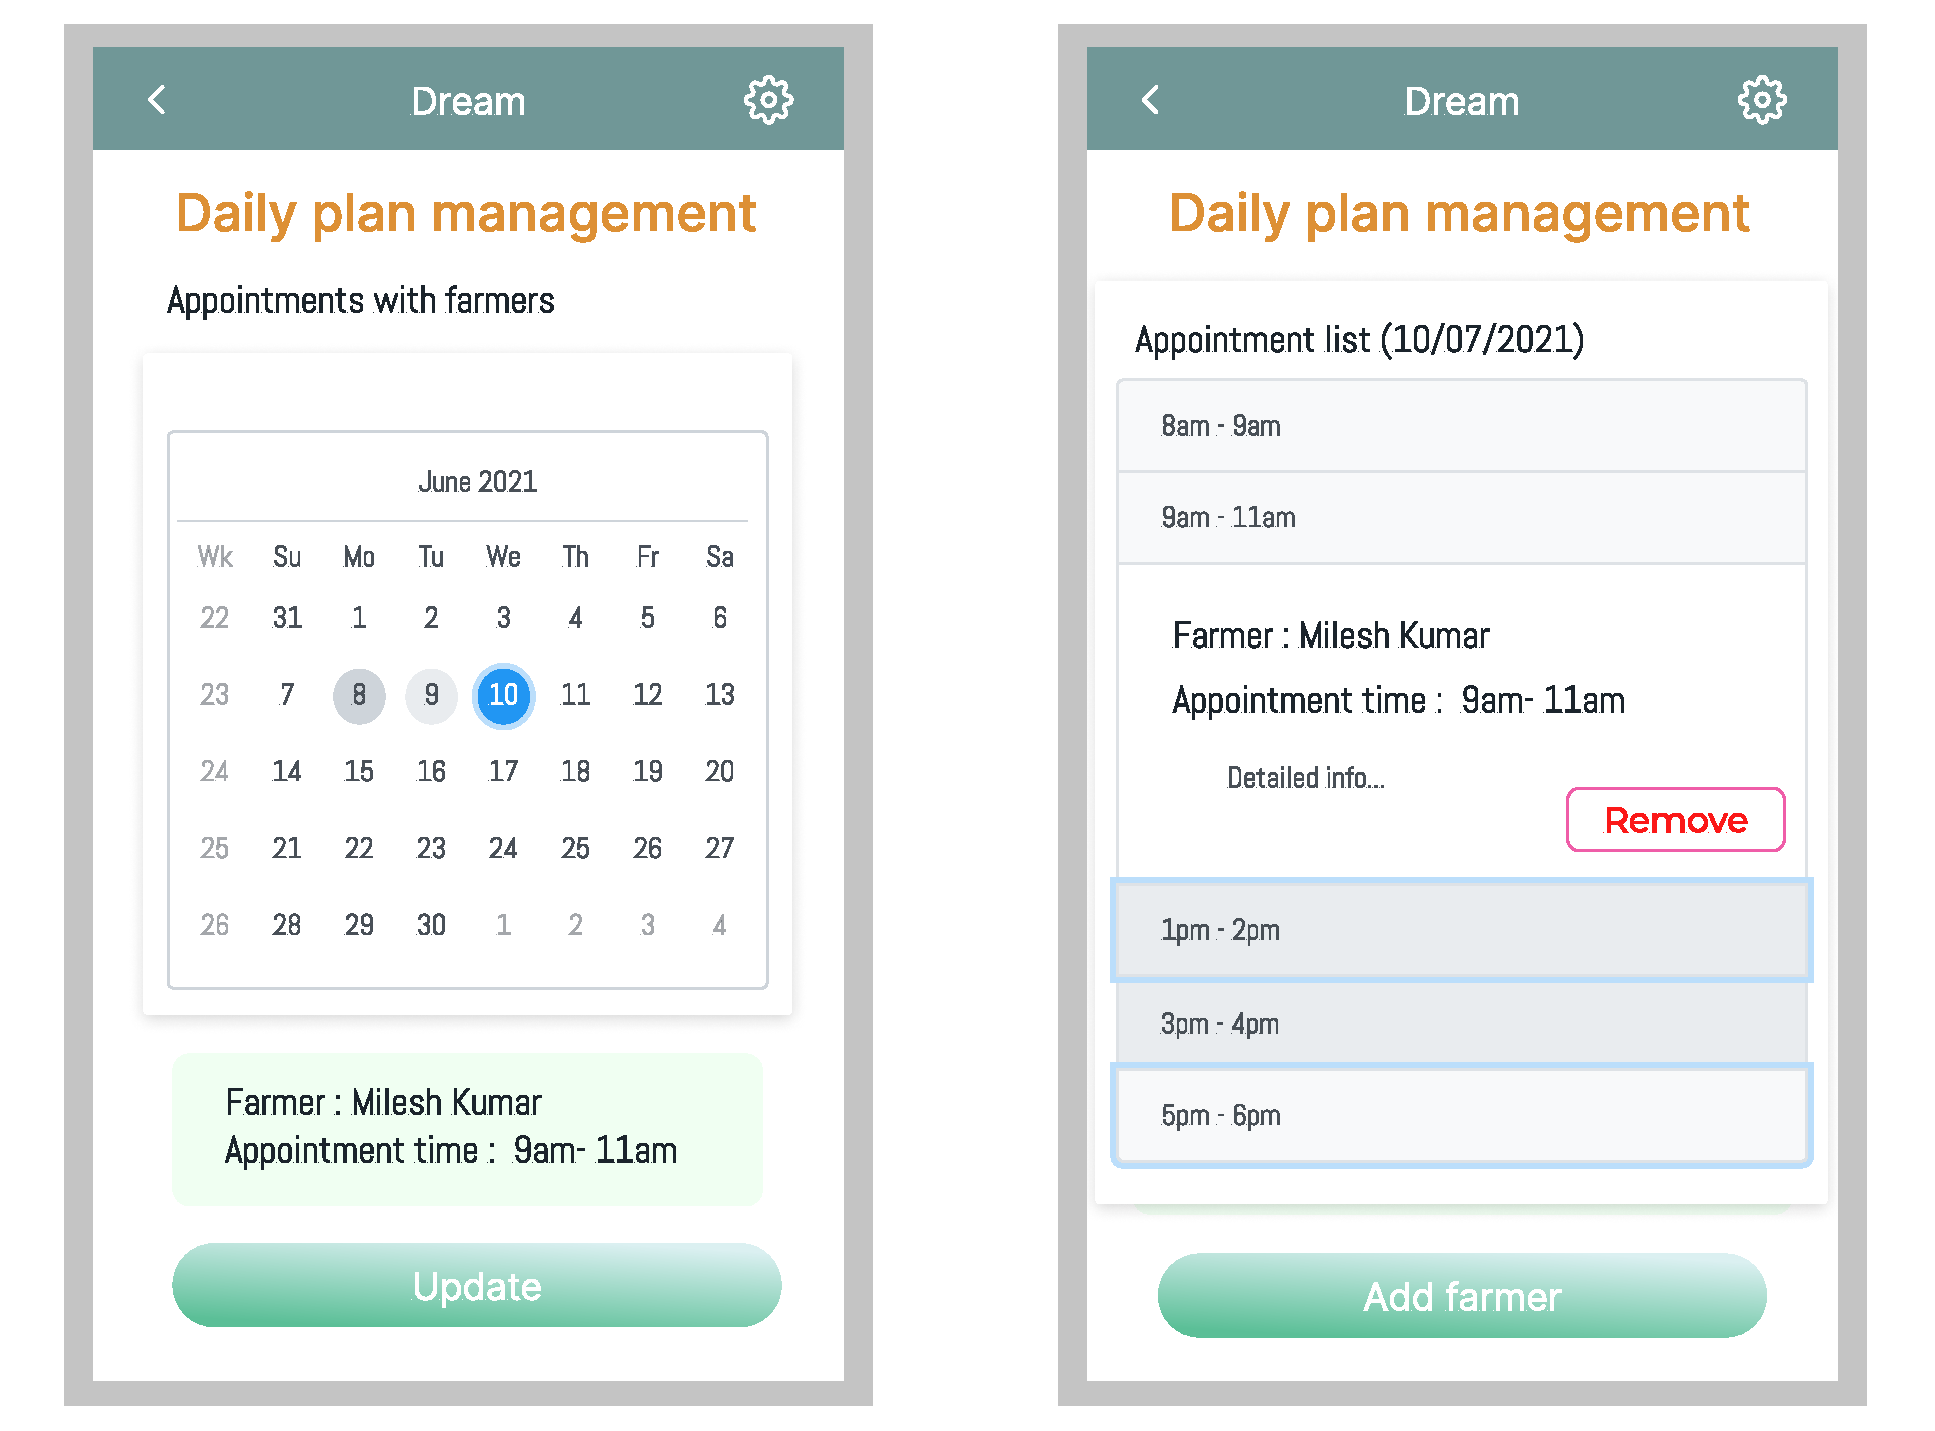
\includegraphics[width=0.8\columnwidth]{Images/UI/daily-plan.pdf}

	\caption{\label{fig:FE_image4}Daily plan update}

\end{figure}

\begin{figure}[H]
	\centering
    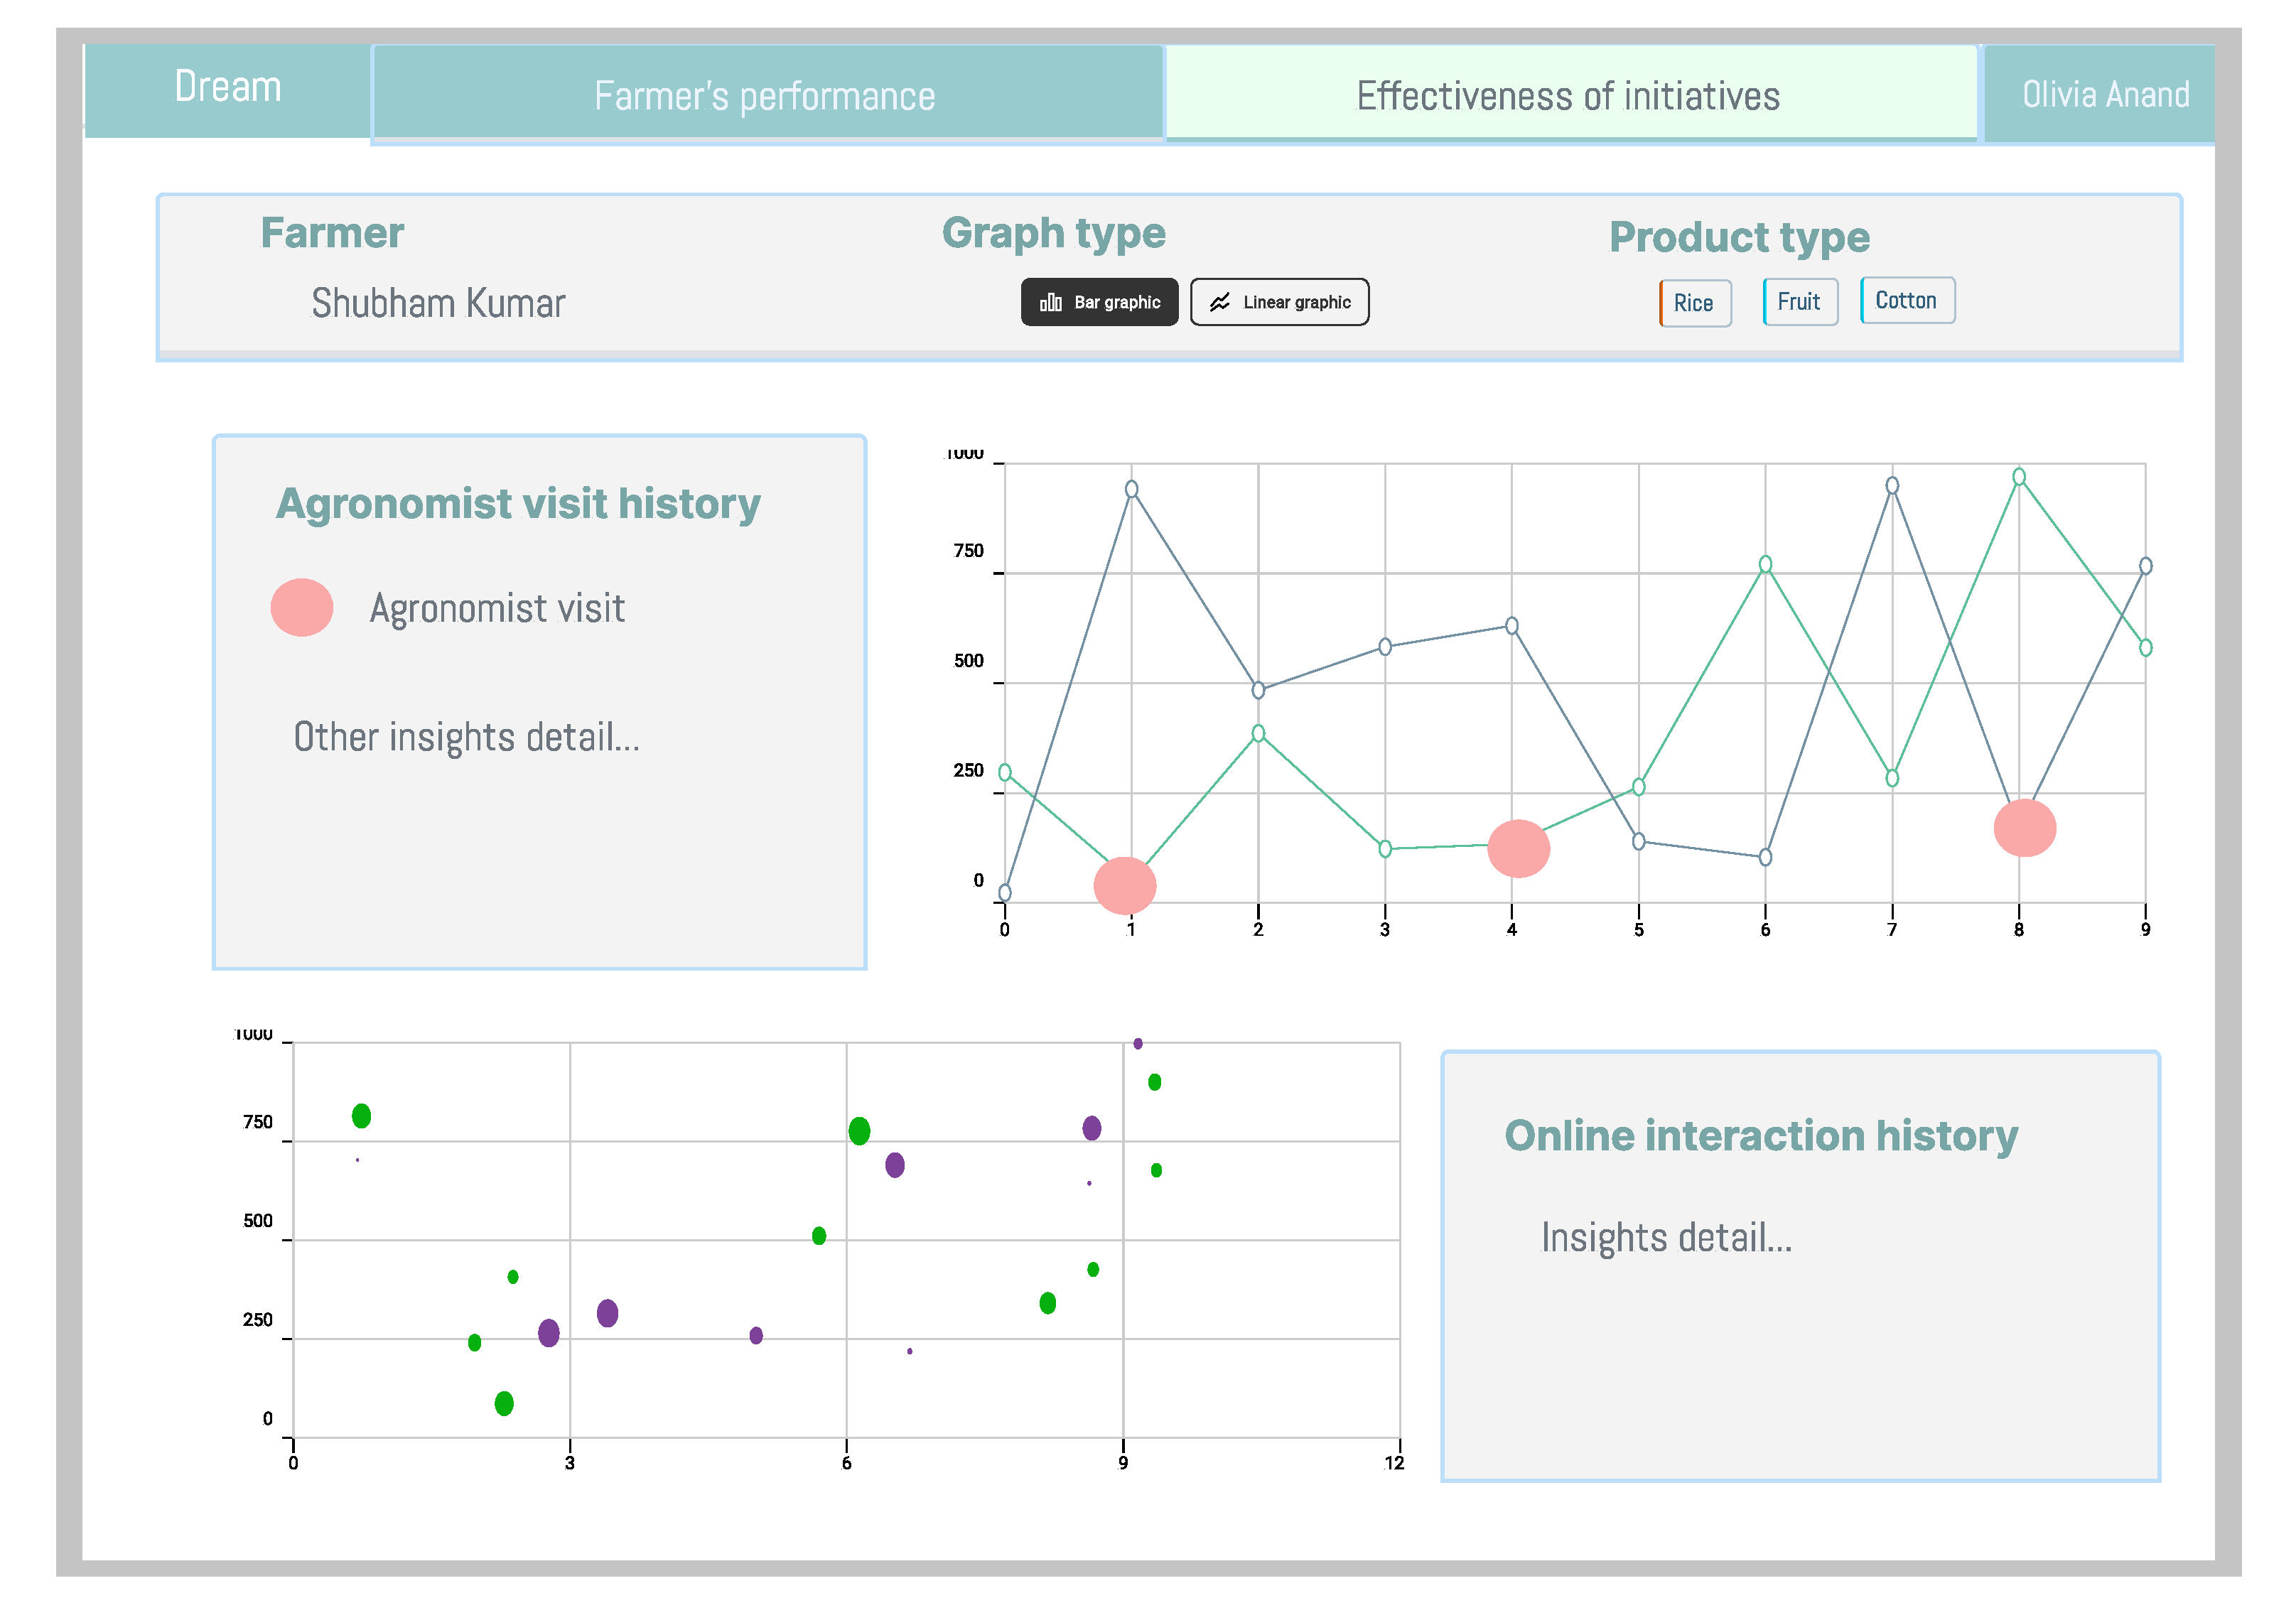
\includegraphics[page=1, width=\textwidth]{Images/UI/effective-initiative.pdf}

	\caption{\label{fig:FE_image5}Effectiveness of initiative}

\end{figure}